\documentclass[11pt]{article}

\usepackage{graphicx}

\begin{document}
\title{CS344 Final: POSIX APIs and their Windows counterparts}
\author{Elliott Capek}
\maketitle

POSIX is a body of rules which specify an interface an operating system can provide to allow programmers to write portable programs. The actual implementation of the interface differs from OS to OS, but any POSIX-adopting OS's interface must have the same behavior. POSIX describes how programs interact with the file system and devices, how processes can access memory, OS information and communicate with each other, how processes can create new processes or threads, and many other things. \\ \\
This document will summarize the following POSIX APIs: memory mapping with \textbf{mmap}, thread creation with \textbf{pthreads}, interprocess communication with \textbf{sockets} and process creating with \textbf{fork}. It will also explain analogous Windows versions of these APIs and how they are different.\\

\section{Sockets}
Sockets are a tool in POSIX that can be used to communicate between processes. A socket is similar to a pipe in that, once two processes have succesfully opened their respective sockets and connected them, reads and writes can be done to the socket and the communication ``just works''. However, this is just one type of socket, known as a Stream Socket. The other major type is called a Datagram Socket, which is different in that individual buffered messages are packaged and sent, and the socket behaves less like a file. A more important difference between sockets and pipes is that sockets are not bound to the same operating system. When a socket is created it is given a protocol to use. The two major ones are the Unix domain and the Inet/Inet6 domain. The former is for communication within the same file system, while the latter is used for communication between networked machines over the internet. Sockets are the major way traffic is sent over the internet. HTTP, SSH, and other important programs/tools use sockets to achieve their inter-machine communication.

\subsection{Sockets in POSIX}
POSIX sockets all have a file descriptor they correspond to. In order to create a new socket for communication, the \textbf{socket(domain, type, protocol)} system call must be used. \textbf{domain} refers to the protocol to be used (local or internet communication). \textbf{type} refers to the type of socket to be used: stream or datagram. Stream sockets are byte-streams. This means that read() and write() calls are used to send messages. Write() blocks until there is enough room in the socket buffer to hold the message. Read blocks until data has been written by the other socket holder. Closing the socket sends an EOF. Reading an EOF also closes the socket. Byte-streams are not conventional files. The lseek() command cannot be used on them, since data is destroyed once it is read. In a byte-stream, there is no concept of ``messages'' - data is written serially. This contrasts with the datagram socket, where messages are passed individually via send and receive calls. Datagram sockets do not guarantee messages are actually sent, or arrive in order. \textbf{protocol} is for future use, and currently has no influence on behavior. It should be 0.\\ \\

\begin{figure}[h!]
\centering
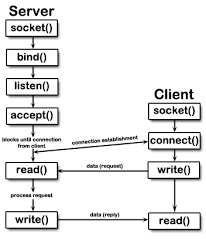
\includegraphics[width=0.5\textwidth]{socket-chronology.png}
\caption{Diagram of chronology of a typical streaming socket connection between a client and server. Image courtesy http://www.cs.uregina.ca/Links/class-info/330/Sockets/sockets.html and ``Unix Network Programming'' by W. Richard Stevens.}
\label{fig:socket-chronology}
\end{figure}

Once a socket has been created, there is a default timeline of events for communication. Typically one process acts as the server, which opens a named socket and waits for a client process to connect. This chronology is shown in Figure (\ref{fig:socket-chronology}). First, \textbf{bind()} is used to give the socket a name. In local communication, this is typically a filename. For internet communication, this is a port. Other processes use this port, along with your computer's host name, to connect. Once the socket is bound, \textbf{listen()} is called to tell the kernel this socket is ready for a connection. After this, two things must happen, and they can happen in any order. The server must \textbf{accept()} a connection request, and a client must initiate a \textbf{connect()} request. The first call blocks until the second call occurs (sort of like a telephone call: one caller blocks until the other answers, or a timeout occurs). The \textbf{accept()} call returns the file descriptor of a new socket which is connected to the client application. Reading and writing (or sending and receiving) can now occur on the two sockets.\\ \\
An interesting thing to note is that in POSIX, a socket is actually two different byte streams: one for reading and one for writing, just like a bidirectional pipe. One process implicitly writes to its write fd and reads from its read fd, even though only one socket file descriptor is used. This behavior is handled by the kernel. \\

\subsection{Sockets in Windows: WinSock}
WinSock, the Windows implementation of sockets, is very similar to the POSIX implementation. There are \textbf{socket()}, \textbf{bind()}, \textbf{listen()}, \textbf{accept()}, \textbf{connect()}, \textbf{recv()} and \textbf{send()} calls which work in a very similar way to the POSIX calls. There are some calls with different names, such as \textbf{closesocket()}. The fact that the \textbf{close()} system call cannot be used on WinSock sockets is a result of WinSock sockets not actually being files, but different sorts of data structures. Windows does not have the ``everything is a file'' paradigm that Unix adopts. This is an advantage in that it puts sockets in a totally different namespace than files, so collisions are less likely. However, it limits users to only using the WinSock API to use sockets, instead of using other APIs to interact with the actual file, like in POSIX. Using non-socket APIs to interact with sockets probably is not very useful, but there may be some cases when it is nice. Another necessary function when using sockets in Windows is the \textbf{WSAStartup()} call, which must be used before any other socket calls are run. This function loads the Windows Sockets DLL (shared library). This is very different than the way POSIX does things, where shared libraries are automatically loaded. This gives more power to the programmer, since it allows them to specify versions and things explicitly. However, it also may cause a performance drop, since DLLs probably take time to load. As expected, the \textbf{WSACleanup()} function must be called after sockets are done being used to unload the DLL.\\

\subsection{POSIX vs Windows: Sockets}
As described above, there are many shared system calls between POSIX and Windows. One of the most notable differences is that, because Windows sockets are not files, \textbf{write()} and \textbf{read()} do not work on Windows sockets. Everything is done through calls to \textbf{recv()} and \textbf{send()}. This allows for less versatility (treating sockets like files makes many things easy in POSIX, like piping a command to a socket) but potentially more confusion, since many of the read() and write() flags used on files do not work on sockets. One thing that is immediately obvious when looking at the MSDS documentation for Windows Sockets is that Windows provides a huge number of socket-specific functions: functions to resolve host names via DNS, simultaneously open and read socket connections, send files over sockets, etc. These are some very powerful API calls that make programming in Windows nice.\\

\section{Memory Mapping}
Memory mapping is the act of creating linkages between regions in a program's memory and external data structures, either files or anonymous spaces in memory. This is incredibly convenient, since it allows programs to write to files as if they were memory (random access via pointers, memset, etc..). It also allows two processes to conveniently share large portions of data, since multiple processes can map their private memory to shared files or anonymous structures. There are two types of mappings: private and shared. The difference is intuitive: only one process can access a private mapping, whereas many processes can access a shared mapping. A private file mapping is a single process taking ownership of a file and using it. If another process maps this file, the kernel assures that changes made by other processes are invisible to to each process. This is actually done by the kernel when allocating a program's text area: a mapping is made in the program's virtual memory to the file holding its binary instructions and the program counter points ot the first instruction. This is used to initialize memory from a file. Private anonymous mappings allocate memory that only the calling process can use. Private anonymous mappings are very similar to malloc() calls. Shared file mappings allow multiple processes to easily and quickly use and modify the same set of data. Shared anonymous mappings use memory that is within the parent process's memory space, and so only children can access it, not other processes.\\ \\

\subsection{POSIX Memory Mapping}
The \textbf{mmap(addr, length, prot, flags, fd, offset)} call is how a memory mapping is created in POSIX. addr is an optional argument (can be NULL) which specifies where the mapping should be created. If null, the kernel decides where the memory will exist. length is the size of the mapping in bytes. prot is a mask specifying whether the memory has read, write and execute permissions. flags specifies whether the mapping is private or shared. flags also specifies whether the mapping is anonymous, whether to clear the anonymous mapping with zeros first, etc. fd and offset are for file mappings (ignored for anonymous mappings) and specify the file descriptor and offset (lseek) of the desired file mapping. The \textbf{munmap()} function does the opposite of mmap.\\ \\

\subsection{Windows Memory Mapping: File Mapping}
As the name implies, the closest analogue of memory mapping in Windows is File Mapping, which only works on files. Windows has a very different jargon than POSIX when it comes to discussing mapping. A File View is an object created by File Mapping that points to a mapped file object in physical memory. A File View is analogous to the data pointer returned by mmap in POSIX. This FV can be written and read to just like a data pointer. Every time the file mapping object is swapped back to the hard drive, the changes are commited to disk. Every File View that points to a file can point to a subsection of the file. FVs are coherent in that changes made in one process are visible to all other processes which map to that same file mapping object. \\ \\
The API for actually creating a file mapping and opening it is fairly different in Windows. You must first call \textbf{CreateFile} to bring the file from disk into memory. This is roughly equivalent to the POSIX \textbf{open()} command. Once you have the file loaded into memory, you must then call \textbf{CreateFileMapping}, which goes ahead and creates a mapped version of the file. Both CreateFile and CreateFile Mapping can both have their own file permissions and sizes, which is unique to Windows. Once a CreateFileMapping object has been made, MapViewOfFile creates the actual file view that the program can use. An FV is basically a data pointer, and can be used almost identically. 

\subsection{POSIX vs Windows: Memory Mapping}
The first major difference between memory mapping and File Mapping is the latter only works on files, not anonymous memory regions. Extra work is likely required to make an anonymous mapping that is not backed up by files on disk. In POSIX, a file is mapped into memory with open(), and this file object has its own permissions and size. mmap() can then be used to map a part of the process's virtual memory into the file, but this mapping has no permissions. It is just a memory object. In Windows, the CreateFile and CreateFile Mapping objects both have different sizes, which is strange. This allows for more flexibility, in that files can be implicitly stretched if not large enough, and processes can be restricted to their own particular part of the file, not necessarily the whole thing. Another difference is that mmap() returns a file pointer, whereas CreateFileMapping objects can create multiple pointers. In C, creating multiple pointers to a mmap() region must be done explicitly. The separation between the file object and the mapped file object in Windows is more complicated, but gives the user more control in that they can restrict a program's access to the file and prevent data collisions. The fact that Windows uses complicated data structures to represent file mappings (instead of just memory regions) gives Windows the ability to set many more features on a memory region, such as its permissions and size. This creates overhead but more power. \\

\section{Threading}
Multithreading is a common element of every modern operating system. Multithreading allows a process to duplicate its program counter, thusly giving it more flexibility, simplifying implementation of asynchronous processes like socket communication, and allowing it to do more work per unit time by having more processor time and possibly running on multple processors at once.\\ \\
For all their power, threads introduce a good deal of danger and complication to a program. Firstly, all threads share the same global data elements. Any time a program is manipulating the same data in two different ways at once without coordination, bad things are bound to happen. This is why threading implementations come with tools to aid in this coordination. There are different threading libraries. This discussion will focus on the \textbf{pthreads} library. pthreads implements a variety of coordination control mechanisms, the first and foremost of which are mutexes and conditional variables.\\ \\
Mutexes are very simple. They are global data elements that store information about the last thread to interact with them. Mutexes provide two operations: locking and unlocking. Locking a mutex ``checks it out'' to your thread, meaning you own it until you ``return'' the mutex by unlocking it. Locking and unlocking must be done in order by a single thread, unlocking of a mutex by a thread that doesn't own it is not permitted. The key feature of mutexes is attempting to lock a mutex causes a thread to block, or stop executing, until it can lock the mutex (ie the thread owning the mutex unlocks it). Mutexes are used to implicitly protect against threads accessing the same data at the same time. According to the mutex honor system, locking a mutex allows a thread to access some data element. Once it is done, the thread unlocks the mutex, loses access to that data, and permits other threads to access it. This means that no threads will simultaneously use a piece of data, since only one thread can own a mutex at any point in time.\\ \\
A conditional variable takes the mutex one step further by adding a signaling feature. A conditional variable is always associated with a mutex. The conditional variable adds a ``signaling'' feature which threads can use to talk to each other. The ``signal'' is like a switch which gets flipped for threads that are waiting for it to be flipped. Just blocking on a lock() call isn't always the answer to thread coordination. Suppose a thread wants to consume a resource that other threads create. Locking a mutex, checking if the resource has been populated, then exiting if it hasn't is slow. Instead, a consumer thread can wait for a conditional variable's signal. That way, it will only lock the mutex when producer threads signal that they have produced a resource to be consumed. \\

\subsection{POSIX pthreads}
The pthreads library has a variety of useful threading functions: \textbf{pthread\_create()}, \textbf{pthread\_start}, \textbf{pthread\_mutex\_lock()}, \textbf{pthread\_mutex\_unlock()}, \textbf{pthread\_cond\_signal()}, and many many more. Threads are identified by their \textbf{thread\_t} id, which is unique to each thread of a process. When a thread is created with \textbf{pthread\_create()}, it is given a thread ID, a starting function (unlike POSIX forking to create new processes, threads have unique starting locations), and arguments. It must then be started via pthread\_start(). pthread mutexes are lock()ed and unlock()ed just as would be expected. Mutexes must be initialized with \textbf{pthread\_mutex\_init()} and destroyed with \textbf{pthread\_mutex\_destroy()}. pthread conditional variables are initialized and destroyed similarly to mutexes. pthreads offers the functions \textbf{pthread\_cond\_wait()} and \textbf{pthread\_cond\_signal()} to use conditional variables to block and signal. \textbf{pthread\_cond\_signal()} does just that: it signals all threads waiting on \textbf{pthread\_cond\_wait()}. \textbf{pthread\_cond\_wait()} has three stages: it first unlock()s the mutex associated with the conditional variable, then it blocks waiting for the signal(), then it relocks the mutex. The surrounding unlock() and lock() calls are there because typically the waiting thread owns the data, then ``lends'' it out to producer threads to do something with, then reclaims it and operates on it.\\

\subsection{Windows Threads}
In the Windows threading library, \textbf{CreateThread} creates threads. This function takes more arguments than the pthreads version. CreateThread allows the user to specify the thread security, the default stack size, and additional creation flags, such as whether to start paused or unpaused. The security of the thread determines whether, when a child is spawned by the process, its children inherit whatever is returned by the thread. Windows also supplies the \textbf{WaitForObject} and \textbf{WaitForMultipleObjects} functions, which are very powerful. They allow the user to block execution until either one or multiple threads are terminated. pthreads has no single function that does this. Windows also implements things like Events, Critical Sections, Interlocking, and a variety of other tools to manage threads. All in all, the Windows threading library is a lot more featureful than the pthreads library. \\

\subsection{POSIX vs Windows: Threading}
The Windows threading API has several features that pthreads does not. First, threads have security levels. This security descriptor allows individual threads to have different rights and permissions, giving them a lot more nuance than the identically-permissioned pthreads threads. Windows threads can also have their initial stack size specified, which gives the user a lot more power over the performance of their programs. Also, Windows threads can either automatically start on creation, or start out paused and be resume()d later. This makes them slightly more powerful than the always-pause-born pthreads threads. The Windows \textbf{WaitForObject} and \textbf{WaitForMultipleObjects} functions are also very powerful. They allow the user to block execution of a main thread until all of its children are done doing their tasks. pthreads does not have anything like this. With pthreads the implementation of this behavior is a lot more complicated, using a conditional variable to signal the main thread that children threads are dead and increment/decrement a counter. Windows has a lot more functions than pthreads does, like functions to manipulate events and critical sections. \\ \\
The basic takeaway message is that pthreads and Windows can do the same things, but Windows makes things much easier. pthreads is perhaps more lightweight, but also requires much more coding to achieve the same effects. This is both a pro and a con. \\

\section{Process Creation}
In POSIX, all processes are children of other processes. Every process descends from another process, up to the progenitor init process. POSIX uses the \textbf{fork()} system call to essentially duplicate a program. Once duplicated, programs are free to modify their program text and execute different code. This is how all processes call other processes. The only difference between a parent process and its children processes immediately after forking is the parent retains its pid, whereas the child process gets a new pid and has its ppid equal to its parent. This is the way child processes differentiate themselves from their parents. Forking in POSIX is efficient because, until a child process changes its program text, it shares the same program text memory area with its parents, since this section is read only. In addition, after forking, the child process actually shares the same memory as its parent. The only difference is once the child attempts to write to this memory, Linux initiates the Copy-on-Write mechanism to duplicate the memory and let the child operate on it as its own separate process. This delayed duplication is efficient because many times a child program doesn't need to modify the heap, only stack variables. Only duplicating if necessary gives the Copy-on-Write mechanism a performance advantage. \\

\subsection{POSIX Process Creation}
\textbf{fork()} is a simple function - it takes no arguments. Once called, a new process is put into the kernel's process queue and begins executing at the same line as the parent process. Once created, both processes need to tell themselves apart, so they examine the output of fork() to see who is who. This child process then typically jumps to a particular function and begins working on something, or it exec()s into a new function to accomplish some task. \\ \\

In addition to the \textbf{execve()} function, POSIX provides many wrapper functions that provide additional functionality than just executing execve(). Some have a built in system() calls which interpret a command string and breaks it up into different function calls and handles piping and redirection. Other flavors of execve wrapper allow simple command names to be given instead of an actual binary executable to be copied. Other options exist as wel. \\ \\

Linux (not POSIX) implements a special \textbf{clone()} function which behaves similarly to fork(), except it allows the user to specify the program's default stack size, starting location and function parameters. It is more powerful than fork(), but usually not necessary since this level of control is not needed. \\

\subsection{Windows Process Creation}
The Windows version of \textbf{fork()}, \textbf{CreateProcess()}, takes many more arguments. CreateProcess allows the user to specify the command line arguments, thread/process handle inheritability, creation flags, environment variables, starting directory pointer and process info structure. This information allows CreateProcess to really customize the child that is being created. Most importantly, CreateProcess allows the user to specify what the new process is going to be. Created processes are not identical copies of the parent, but have their own program text off the bat.

\subsection{POSIX vs Windows: Process Creation}
CreateProcess is a much heavier function - it takes infinitely more arguments than fork()! As is the usual Windows implementation, CreateProcess gives the user all the control up front in a large function call. The advantage of this is that it allows lots of customization up front, especially if all the user is doing is creating a new process to run a certain program, like ``dir.'' However, the advantage of the fork() then execve() approach of POSIX is that it allows for much more creativity and varied behavior. If the child process is to run the same program as the parent, just a different function inside it, then fork() without execve() is an efficient way to handle this, due to the kernel's Copy-on-Write mechanism. CreateProcess doesn't have an easy way to do this, it always spawns a new process. While the same tasks are accomplishable in either system, the POSIX way usually involves more coding. However, forcing the user to write all this code can be good, since it forces everything to be done properly. The difference between the two calls isn't that large. Windows provides a lot more options for security and customizability, but the POSIX implementation is easier to use. 

\section{Sources}

Rose, Johnnie. "Johnnie's Winsock Tutorial by Johnnie Rose, Jr." \textit{Johnnie's Winsock Tutorial by Johnnie Rose, Jr.} Web. 15 Aug. 2015.\\
http://johnnie.jerrata.com/winsocktutorial/. \\ \\

MSDN Socket Documentation. Web. 14 Aug. 2015.\\
https://msdn.microsoft.com/en-us/library/windows/desktop/ms740632(v=vs.85).aspx \\ \\

MSDN Threading Documentation. Web. 14 Aug. 2015. \\
https://msdn.microsoft.com/en-us/library/aa366556(VS.85).aspx \\ \\

MSDN Process Creation Documentation. Web. 14 Aug. 2015. \\
https://msdn.microsoft.com/en-us/library/windows/desktop/ms684863(v=vs.85).aspx \\ \\

Kerrisk, Michael. \textit{The Linux Programming Interface a Linux and UNIX System Programming Handbook}. San Francisco: No Starch, 2010. Print.

\end{document}
